\section{Discriminant pairings and the number of admissible columns}
\label{sec:pairings}

We now relate the size of \(\mathcal S_{L_0}(B)\) to the cyclic
factors of the finite group \(G_B=\Z^m/B\Z^m\). The estimate
will apply when the factors beyond the two largest in each primary
component have small total logarithmic size. Layers provide convenient
notation for this condition.

\subsection{Layers and the static estimate}

For a finite abelian group \(G\), write its \(l\)-primary part as
\[
 G_l\cong\bigoplus_i\Z/l^{b_{l,i}}\Z,
 \qquad b_{l,1}\ge b_{l,2}\ge\cdots\ge0,
\]
where \(l\) always denotes a prime and zero exponents are appended.
For \(j\ge1\), define the \emph{layer height} and its weight by
\[
 k_G(l,j)=\#\{i:b_{l,i}\ge j\},
 \qquad \nu_l=\frac{\log_N l}{N}.
\]
A layer is a pair \((l,j)\) of positive height. Write \(k_B\) for
\(k_{G_B}\). For \(G_B\), and for every quotient of \(G_B\),
Hadamard's inequality gives
\begin{equation}\label{eq:group-order}
 \sum_{l,j}k_G(l,j)\nu_l
 =\frac{\log_N|G|}{N}\le\frac12,
 \qquad m\le N.
\end{equation}
Indeed, \(|G|\le|\det B|\le m^{m/2}\le N^{N/2}\).
The trivial group has no layers, so its sums are zero.

For \(s\ge0\), define
\begin{equation}\label{eq:tail-potential}
 W_s(B)=\sum_{l,j}(k_B(l,j)-s)_+\nu_l,
 \qquad (x)_+=\max\{x,0\}.
\end{equation}
Two related quantities will distinguish the two cases of the proof:
\begin{equation}\label{eq:pairing-weights}
 T_2(B)=\sum_{k_B(l,j)=2}\nu_l
       =\sum_l(b_{l,2}-b_{l,3})\nu_l,
 \qquad
 J_B=\sum_{k_B(l,j)\ge3}k_B(l,j)\nu_l.
\end{equation}
Thus \(T_2\) counts layers of height exactly two, whereas \(J_B\)
counts their full heights when the height is at least three.
In particular,
\begin{equation}\label{eq:pairing-high-tail}
 0\le J_B\le\frac12,
 \qquad J_B\le3W_2(B),
\end{equation}
since \(k\le3(k-2)\) for every integer \(k\ge3\).
Figure~\ref{fig:layers} illustrates these distinctions at one prime.

\begin{figure}[H]
 \centering
 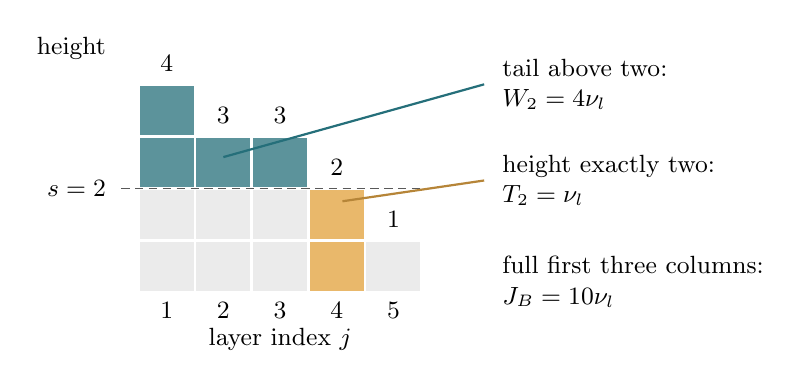
\begin{tikzpicture}[x=0.72cm,y=0.66cm,font=\small]
 \definecolor{layertail}{RGB}{37,111,122}
 \definecolor{layertwo}{RGB}{227,166,70}
 \foreach \j/\height in {1/4,2/3,3/3,4/2,5/1} {
  \foreach \i in {1,...,\height} {
   \fill[black!8] (\j-1,\i-1) rectangle (\j,\i);
   \ifnum\i>2
    \fill[layertail!75] (\j-1,\i-1) rectangle (\j,\i);
   \fi
   \ifnum\j=4
    \fill[layertwo!80] (\j-1,\i-1) rectangle (\j,\i);
   \fi
   \draw[white,line width=1pt] (\j-1,\i-1) rectangle (\j,\i);
  }
  \node[below] at (\j-0.5,0) {\(\j\)};
  \node[above] at (\j-0.5,\height+0.05) {\(\height\)};
 }
 \draw[densely dashed,black!65] (-0.3,2)--(5.3,2);
 \node[anchor=east] at (-0.4,2) {\(s=2\)};
 \node[anchor=east] at (-0.4,4.7) {height};
 \node at (2.5,-0.9) {layer index \(j\)};
 \draw[layertail,thick] (1.5,2.6)--(6.1,4.0);
 \node[anchor=west,align=left] at (6.25,4.0)
   {tail above two:\\ \(W_2=4\nu_l\)};
 \draw[layertwo!80!black,thick] (3.6,1.75)--(6.1,2.15);
 \node[anchor=west,align=left] at (6.25,2.15)
   {height exactly two:\\ \(T_2=\nu_l\)};
 \node[anchor=west,align=left] at (6.25,0.2)
   {full first three columns:\\ \(J_B=10\nu_l\)};
\end{tikzpicture}

 \caption{Layers for a primary group with cyclic exponents
 \((5,4,3,1)\). The column heights are \((4,3,3,2,1)\).
 \(W_2\) and \(J_B\) count selected squares, each of weight
 \(\nu_l\), while \(T_2\) counts each height-two column once.
 The four dark squares above the
 dashed cutoff contribute \(4\nu_l\) to \(W_2\). The orange column
 is the unique layer of height exactly two, contributing \(\nu_l\)
 to \(T_2\). The first three columns have total weight \(10\nu_l\)
 and contribute that amount to \(J_B\).}
 \label{fig:layers}
\end{figure}

We use the slowly varying scales
\begin{equation}\label{eq:layer-scales}
 R=\lceil\ell^2\rceil,
 \qquad \sigma=R^{-6}.
\end{equation}
They will also be used in Section~\ref{sec:paths}.

\begin{proposition}[Static column estimate]\label{prop:static-column}
For every fixed \(L_0\ge1\) and \(e_0>0\), there is a fixed
\(\zeta>0\) such that, typically for nonsingular bit matrices
\(B\) of size \(m\in\mathcal I_N\),
\[
 W_2(B)\le\zeta
 \quad\Longrightarrow\quad
 |\mathcal S_{L_0}(B)|\le2^{e_0N}.
\]
\end{proposition}

The proposition leaves matrices with large \(W_2\) for the path
argument. Its proof separates according to \(T_2\). Layers of height
exactly two can force admissible columns into a few subgroups of large
index; Theorem~\ref{thm:small-intersection} then applies. Otherwise
a coloring controls the pairing on differences of columns. An
arithmetic determinant bound and the spectrum of \(B\) then bound
the dimension of a large subset of one color. We first develop the
pairing argument that distinguishes these two cases.

\subsection{Colors and subgroups of large index}

The \emph{discriminant pairing} of \(B\) is
\begin{equation}\label{eq:discriminant-pairing}
 \lambda_B(\bar x,\bar y)
   =x^{\mathsf T}B^{-1}y\bmod\Z,
 \qquad \bar x,\bar y\in G_B.
\end{equation}
It is well defined because changing either representative by an
integer column combination of \(B\) changes the value by an integer.
It is \emph{perfect}: the map
\(G_B\to\operatorname{Hom}(G_B,\Q/\Z)\) defined by the pairing
is an isomorphism. To see injectivity, an element pairing to zero
with every coordinate class satisfies \(B^{-1}x\in\Z^m\), so its
class is zero; the two finite groups have equal order.
Distinct primary components are orthogonal, since their mutual
pairing is annihilated by coprime powers. An element is called
\emph{isotropic} if its self-pairing is zero. Every
\(z\in\mathcal S_{L_0}(B)\) has isotropic class, and its primary
components are individually isotropic by uniqueness of primary
decomposition in \(\Q/\Z\).

The orthogonal block decomposition of a perfect primary pairing
uses cyclic blocks and, at \(l=2\), possible two-generator blocks
with equal cyclic exponents. These decompositions are classical;
see Miranda~\cite[Section~1]{Miranda}. We use the following precise
consequences of the decomposition and the coloring analysis in
\cite[Lemmas 6.1--6.3]{SymmetricRate}.

\begin{lemma}[Coloring input]\label{lem:pairing-colors}
Let \(B\) be a nonsingular symmetric integer matrix. For each prime
\(l\), put \(f_l=b_{l,3}\). The perfect pairing on \(G_{B,l}\)
admits an orthogonal decomposition
\[
 G_{B,l}=U_l\oplus V_l,
\]
where \(U_l\) consists of the blocks with cyclic exponents strictly
greater than \(f_l\), and the exponent of \(V_l\) divides
\(l^{f_l}\). There are at most two cyclic factors in \(U_l\).
The isotropic elements of \(G_{B,l}\) can be colored with \(C_l\)
colors satisfying
\begin{equation}\label{eq:primary-color-count}
 C_l\le1+8b_{l,1},
 \qquad C_l\le2^{b_{l,2}-b_{l,3}}\quad\text{if \(l\) is odd},
\end{equation}
such that two elements of one color satisfy
\begin{equation}\label{eq:primary-color-pairing}
 l^{f_l}\lambda_B(x_{U_l},y_{U_l})=0
 \quad\text{in }\Q/\Z.
\end{equation}
If \(X\subset G_B\) consists of isotropic elements with one fixed
color at every prime, put \(H=\langle x-y:x,y\in X\rangle\).
Then the image of the \emph{restricted} pairing map
\begin{equation}\label{eq:restricted-pairing-map}
 H\longrightarrow\operatorname{Hom}(H,\Q/\Z),
 \qquad u\longmapsto\lambda_B(u,\cdot)|_H,
\end{equation}
has order at most \(N^{NJ_B}\).
\end{lemma}

The cutoff in Lemma~\ref{lem:pairing-colors} does not split a
block, since the two exponents in each two-generator block are equal.
The restriction in
Equation~\eqref{eq:restricted-pairing-map} is essential: the
characters are tested on \(H\), not on all of \(G_B\).

For our purposes the same coloring has another consequence.

\begin{lemma}[A subgroup containing each color]\label{lem:color-subgroup}
For every prime \(l\), each primary color in
Lemma~\ref{lem:pairing-colors} is contained in a subgroup of
\(G_{B,l}\) whose index is at least
\(l^{b_{l,2}-b_{l,3}}\).
\end{lemma}

\begin{proof}
Write \(f=f_l\) and \(U=U_l\). Multiply the perfect pairing on
\(U\) by \(l^f\), and quotient \(U\) by the radical of this
new pairing. The resulting pairing on a group \(\bar U\) is
perfect. Its order is
\[
 |\bar U|=l^{\sum_i(b_{l,i}-f)_+}.
\]
Indeed, under the original perfect pairing the new radical is
\(U[l^f]=\{u\in U:l^fu=0\}\), and each cyclic factor of exponent
\(b>f\) leaves a quotient of order \(l^{b-f}\).
By Equation~\eqref{eq:primary-color-pairing}, the images of one
color generate a subgroup \(A\subset\bar U\) with
\(A\subset A^\perp\). Perfectness gives
\(|A|\,|A^\perp|=|\bar U|\), so
\[
 [\bar U:A]\ge|\bar U|^{1/2}
 =l^{\frac12\sum_i(b_{l,i}-f)_+}
 \ge l^{b_{l,2}-f}.
\]
Take the preimage of \(A\) in \(U\), and add the unrestricted
summand \(V_l\). This subgroup contains the entire primary color
and has the required index. The argument also covers \(U=0\),
when the asserted index is one.
\end{proof}

The next counting step controls the price of specifying colors. It
uses both bounds in Equation~\eqref{eq:primary-color-count}: the
odd-prime bound is efficient before a weight threshold is reached,
and the polynomial bound controls the prime that crosses it.

\begin{lemma}[Cost of specifying colors]\label{lem:color-cost}
Uniformly over nonsingular symmetric bit matrices of size at most
\(N\), the following hold as \(N\to\infty\).
\begin{enumerate}[label=\textup{(\roman*)}]
 \item If \(T_2(B)\ge\sigma\), there is a set of primes
 \(\mathcal P\) such that
 \[
  \sum_{l\in\mathcal P}(b_{l,2}-b_{l,3})\nu_l\ge\sigma,
  \qquad \sum_{l\in\mathcal P}\log_2 C_l=o(N).
 \]
 \item If \(T_2(B)<\sigma\), then
 \(\sum_l\log_2 C_l=o(N)\).
\end{enumerate}
\end{lemma}

\begin{proof}
The group-order bound gives
\(b_{l,1}\le(N/2)\log_2N\), so the first bound in
Equation~\eqref{eq:primary-color-count} costs \(O(\log N)\) bits
per prime. All primes \(l\le\sqrt N\) together therefore cost
\(O(\sqrt N\log N)=o(N)\).
For larger primes, \(\nu_l>1/(2N)\); they are odd for large
\(N\), and hence
\begin{equation}\label{eq:large-prime-color-cost}
 \sum_{l\in\mathcal P,\ l>\sqrt N}\log_2 C_l
 \le\sum_{l\in\mathcal P,\ l>\sqrt N}(b_{l,2}-b_{l,3})
 \le2N\sum_{l\in\mathcal P,\ l>\sqrt N}
                 (b_{l,2}-b_{l,3})\nu_l.
\end{equation}
For \textup{(i)}, first include every contributing prime at most
\(\sqrt N\). If their total weight is below \(\sigma\), add
larger contributing primes until that threshold is first reached.
Before the last prime, Equation~\eqref{eq:large-prime-color-cost}
costs at most \(2\sigma N\) bits. Charge the last prime only
\(O(\log N)\) bits using the first color bound, regardless of
its weight. The total is \(o(N)\), since \(\sigma\to0\).
For \textup{(ii)}, Equation~\eqref{eq:large-prime-color-cost}
applies to all large primes with total cost at most
\(2\sigma N\); the small-prime cost is unchanged.
\end{proof}

Fix \(0<\alpha<\min\{e_0,1\}\), and impose the typical event of
Theorem~\ref{thm:small-intersection} with \(D=20\). Since
\(\tau=\ell^{-20}=o(\sigma)\), the preceding lemmas settle all
matrices with \(T_2(B)\ge\sigma\). In fact, specify colors only
at the primes selected in Lemma~\ref{lem:color-cost}\textup{(i)}.
There are \(2^{o(N)}\) resulting parts of
\(\mathcal S_{L_0}(B)\). By Lemma~\ref{lem:color-subgroup}, each
part lies in the preimage \(K\subset\Z^m\) of a subgroup of
\(G_B\) with
\[
 B\Z^m\subset K\subset\Z^m,
 \qquad [\Z^m:K]\ge N^{\sigma N}\ge N^{\tau N}.
\]
Theorem~\ref{thm:small-intersection} bounds its size by
\(2^{\alpha N}\). Consequently
\begin{equation}\label{eq:height-two-columns}
 |\mathcal S_{L_0}(B)|\le2^{\alpha N+o(N)}\le2^{e_0N}
\end{equation}
for sufficiently large \(N\). This argument uses the theorem's
simultaneity over all lattices: the color subgroups may depend on
\(B\).

\subsection{A lattice of graph differences}

It remains to control the column set when \(T_2(B)<\sigma\).
The color cost is then subexponential. We first show how two
real-matrix estimates would bound the dimension of a large part of
one color; their probabilistic proofs will follow the comparison.

A nonempty finite set \(\mathcal A\) is \emph{\(\rho\)-robust}
on its affine span \(F\) if every affine subspace \(E\subset F\)
of codimension \(t\) satisfies
\[
 |\mathcal A\cap E|\le2^{-\rho t}|\mathcal A|.
\]
We use the following two geometric inputs from
\cite[Lemmas 3.7 and 3.8]{SymmetricRate}.

\begin{lemma}[Robust extraction]\label{lem:robust-extraction}
If \(\varnothing\ne\mathcal A\subset\bits^m\) and \(\rho>0\),
there is an affine subspace \(E\) for which the nonempty set
\(\mathcal V=\mathcal A\cap E\) is \(\rho\)-robust on its affine
span and satisfies
\[
 \log_2|\mathcal V|\ge\log_2|\mathcal A|-\rho m.
\]
\end{lemma}

\begin{lemma}[Determinant of a robust image lattice]\label{lem:robust-image}
Fix \(D,C_0>0\) and put \(\rho=\ell^{-D}\). Let
\(\varnothing\ne\mathcal V\subset\bits^m\), \(m\le N\), be
\(\rho\)-robust on its affine span \(F\), of dimension \(r\).
Let \(\Phi:F\to\R^d\) be an injective rational affine map such that
\[
 \lVert\Phi(v)-\Phi(w)\rVert_2\le C_0\sqrt N
 \qquad(v,w\in\mathcal V).
\]
Then the integer span of its image differences is a rank-\(r\)
lattice of covolume at most \(\exp(O_{D,C_0}(N\ell))\).
Also
\(H(\Span(\mathcal V-\mathcal V))\le\exp(O_D(N\ell))\).
The covolumes in rank zero are one.
\end{lemma}

For a symmetric matrix \(C\) and a linear subspace
\(F\subseteq\R^m\), the notation \(C|_F\) denotes the
restriction of its bilinear form to \(F\times F\), rather than the
restriction of the associated linear map. Its radical is
\[
 \rad(C|_F)=\{x\in F:x^{\mathsf T}Cy=0\text{ for every }y\in F\}.
\]
Its dimension is the nullity \(\dim F-\rank(C|_F)\).

We will also use a determinant consequence of a finite pairing
image. We include its short proof to make clear why the image order
enters to the first power; this is
\cite[Lemma 6.4]{SymmetricRate}.

\begin{lemma}[Pairing image and determinant]\label{lem:pairing-determinant}
Let \(L\) be a lattice spanning a Euclidean space \(V\), and let
\(q\) be a symmetric bilinear form with \(q(L,L)\subset\Q\).
Set
\[
 K=L\cap\rad q,
 \qquad S=V\cap(\rad q)^\perp.
\]
If the image of \(L\to\operatorname{Hom}(L,\Q/\Z)\),
\(x\mapsto q(x,\cdot)\bmod\Z\), has order \(t\), then
\begin{equation}\label{eq:pairing-det}
 |\det_{\mathrm{orth}}(q|_S)|
 \ge\frac{(\det K)^2}{t(\det L)^2}.
\end{equation}
The determinant on the left is in an orthonormal basis of \(S\).
\end{lemma}

\begin{proof}
The matrix of \(q\) in a lattice basis is rational. Its radical
therefore has a rational basis, so \(K\) spans the radical and is
primitive in \(L\). The orthogonal projection \(\bar L\) of
\(L\) onto \(S\) is a lattice, and
\(\det L=\det K\det\bar L\). The form descends to \(\bar L\)
with the same pairing image order, because pullback of characters
along \(L\to\bar L\) is injective.

Let \(M\) be the nonsingular matrix of the descended form in a
basis of \(\bar L\). Its pairing kernel modulo \(\Z\) in the
coordinate lattice has index \(t\). If \(A\) is an integer basis
matrix for that kernel, then \(|\det A|=t\) and
\(A^{\mathsf T}M\) is integral and nonsingular. Thus
\[
 1\le|\det(A^{\mathsf T}M)|=t|\det M|.
\]
Changing from the lattice basis to an orthonormal basis divides
this determinant by \((\det\bar L)^2\), which proves
Equation~\eqref{eq:pairing-det}. If \(S\) has dimension zero, then \(K=L\) and \(t=1\),
so both sides of Equation~\eqref{eq:pairing-det} are one.
\end{proof}


\begin{lemma}[The graph comparison]\label{lem:graph-comparison}
Fix \(L_0\ge1\) and \(\xi,w>0\). Suppose that \(B\) is a
nonsingular symmetric bit matrix of size \(m\in\mathcal I_N\),
with \(T_2(B)<\sigma\), and that the following hold:
\begin{enumerate}[label=\textup{(\roman*)}]
 \item for every rational \(F\subseteq\R^m\) of height at most
 \(\exp(N\ell^2)\),
 \(\rank(B^{-1}|_F)\ge\dim F-\xi N\);
 \item at most \(\xi N\) eigenvalues of \(B\) lie in
 \([-w\sqrt N,w\sqrt N]\).
\end{enumerate}
Then
\[
 |\mathcal S_{L_0}(B)|\le 2^{(2J_B+2\xi+o(1))N},
\]
where the error tends to zero uniformly over these matrices, for
fixed \(L_0,\xi,w\).
\end{lemma}

\begin{proof}
The assertion is immediate if \(\mathcal S_{L_0}(B)\) is empty.
Choose a largest overall color \(\mathcal A\) of the column set,
and apply Lemma~\ref{lem:robust-extraction} with
\(\rho=\ell^{-2}\). For the resulting set \(\mathcal V\),
Lemma~\ref{lem:color-cost}\textup{(ii)} gives
\begin{equation}\label{eq:robust-column-size}
 \log_2|\mathcal S_{L_0}(B)|
 \le\log_2|\mathcal V|+o(N).
\end{equation}
Put \(F_0=\Span(\mathcal V-\mathcal V)\) and
\(r_0=\dim F_0\). We place each column beside its inverse
image: the norm condition keeps differences short, while the first
coordinates remain integral. The induced graph metric will also
control the inverse form near small eigenvalues of \(B\). Define
the rational graph map and its difference lattice
\[
 \gamma(x)=(x,B^{-1}x),\qquad
 L=\langle\gamma(v)-\gamma(v'):v,v'\in\mathcal V\rangle_{\Z}
       \subset\gamma(F_0).
\]
The graph differences satisfy
\[
 \lVert\gamma(v)-\gamma(v')\rVert_2^2
 \le m+4L_0^2N\le(1+4L_0^2)N.
\]
Lemma~\ref{lem:robust-image}, applied both to the graph map and
to the identity map, consequently gives
\begin{equation}\label{eq:graph-height}
 \det L\le\exp(O_{L_0}(N\ell)),
 \qquad H(F_0)\le\exp(O(N\ell))\le\exp(N\ell^2)
\end{equation}
for sufficiently large \(N\).

On the full graph \(\Gamma=\gamma(\R^m)\), define the rational
symmetric form
\[
 q(\gamma(x),\gamma(y))=x^{\mathsf T}B^{-1}y.
\]
Its restriction to \(\gamma(F_0)\) has rank \(s\) satisfying
\begin{equation}\label{eq:graph-rank}
 s\ge r_0-\xi N
\end{equation}
by the first hypothesis and Equation~\eqref{eq:graph-height}.
The hypothesis covers every subspace of this height, including
\(F_0\), which was selected from admissible columns for \(B\).

The map \(L\to G_B\) taking \(\gamma(u)\) to \(u+B\Z^m\)
has image
\[
 H=\langle\bar v-\bar v':v,v'\in\mathcal V\rangle.
\]
It is surjective onto \(H\), and the form modulo \(\Z\) is the
pullback of the restricted pairing on \(H\). Pullback of characters
is injective, so the two pairing maps have equal image orders.
Lemma~\ref{lem:pairing-colors} bounds this order by \(N^{NJ_B}\).
Let \(K\) be the radical lattice of the restriction to
\(\gamma(F_0)\), and let \(S\) be its radical's orthogonal
complement in that space. The first-coordinate projection is
injective on \(\Gamma\) and takes \(K\) to an integer lattice
of the same rank. Such a lattice has covolume at least one, and
orthogonal projection contracts volumes. Hence \(\det K\ge1\).
Lemma~\ref{lem:pairing-determinant} now yields
\begin{equation}\label{eq:graph-det-lower}
 |\det_{\mathrm{orth}}(q|_S)|
 \ge N^{-NJ_B}\exp(-O_{L_0}(N\ell)).
\end{equation}

The same determinant admits an upper bound from the spectrum of
\(B\). If \(v\) is a unit eigenvector with nonzero eigenvalue
\(x\), its graph vector has squared norm \(1+x^{-2}\), while
\(q(\gamma(v),\gamma(v))=x^{-1}\). Orthogonal eigenvectors of
\(B\) have orthogonal graph vectors. Thus the eigenvalues of the
self-adjoint operator representing \(q\) on \(\Gamma\) are
\[
 \frac{x}{1+x^2}.
\]
They have absolute value at most one. By the second hypothesis,
all but at most \(\xi N\) of them have absolute value at most
\(C_w/\sqrt N\), where \(C_w=1/w\).

The absolute determinant of the compression of a self-adjoint
operator to any \(s\)-dimensional subspace is at most the product
of its largest \(s\) singular values. Indeed, it is
\(\langle\omega,(\bigwedge^s T)\omega\rangle\), where \(\omega\) is the
unit exterior product of an orthonormal basis of the subspace.
Applying this to \(S\), whose dimension is \(s\), gives
\begin{equation}\label{eq:graph-det-upper}
 |\det_{\mathrm{orth}}(q|_S)|
 \le\left(\frac{C_w}{\sqrt N}\right)^{(s-\xi N)_+}.
\end{equation}
This argument applies to indefinite forms and includes \(s=0\).
Combining Equations~\eqref{eq:graph-det-lower}
and~\eqref{eq:graph-det-upper}, and then using
Equation~\eqref{eq:graph-rank}, gives
\[
 (s-\xi N)_+
   \left(\frac12\log N-\log C_w\right)
 \le NJ_B\log N+O_{L_0}(N\ell),
 \qquad
 \frac{r_0}{N}\le2J_B+2\xi+o(1).
\]
The second bound also holds when \(s<\xi N\).

Finally, projection to \(r_0\) suitable coordinates is injective
on the affine span of \(\mathcal V\), so
\(|\mathcal V|\le2^{r_0}\). Equation~\eqref{eq:robust-column-size} and the preceding
dimension bound imply
\[
 \frac1N\log_2|\mathcal S_{L_0}(B)|
 \le 2J_B+2\xi+o(1).
\]
The error is bounded by
\(O_{L_0,w}(\ell^{-2}+\sigma+N^{-1/2}\log N+\ell/\log N)\).
The first three terms come from extraction and colors, and the last
from the determinant comparison, using \(J_B\le1/2\). This
establishes the asserted uniformity.
\end{proof}

\subsection{Uniform rank and spectral estimates}

Lemma~\ref{lem:graph-comparison} identifies the two remaining
probabilistic requirements: inverse forms must retain rank on every
low-height span, and most eigenvalues must stay away from zero at
scale \(\sqrt N\). We now verify both requirements for the biased
bit model. The arguments adapt
\cite[Corollary~5.2 and Proposition~5.4]{SymmetricRate} to the biased
arrays. The rank estimate uses the atom bound \(b\); the spectral
estimate uses the common variance \(pb\) and the rank-two bound
on the mean.

\subsubsection{Inverse forms on low-height subspaces}

\begin{proposition}[Uniform inverse restriction rank]
\label{prop:inverse-rank}
For every fixed \(D>0\) and \(\xi>0\), typically every nonsingular bit
matrix \(B\) satisfies, simultaneously for all rational subspaces
\(F\subseteq\R^m\) with \(H(F)\le\exp(N\ell^D)\),
\[
 \rank(B^{-1}|_F)\ge\dim F-\xi N.
\]
\end{proposition}

\begin{proof}
First fix an arbitrary real subspace \(U\subseteq\R^m\) of dimension
\(d\). Choose a basis matrix \(V\) and a coordinate set \(I\) of size
\(d\) so that \(V_I\) is the identity matrix. Conditional on all
entries of \(B\) outside the principal block \(I\times I\), the
matrix of \(B|_U\) in this basis is
\[
 V^{\mathsf T}BV=B_{I,I}+H,
\]
where \(H\) is a fixed symmetric matrix. The unrevealed entries of
\(B_{I,I}\) are independent bits, each with largest atom \(b\).
Equation~\eqref{eq:typical-corank-tail} therefore shows that
\begin{equation}\label{eq:fixed-restriction-tail}
 \Prob\bigl(\dim\rad(B|_U)\ge\lceil\xi N/2\rceil\bigr)
 \le 2^{-c_{p,\xi}N^2}
\end{equation}
for all sufficiently large \(N\); the event is empty if
\(d<\lceil\xi N/2\rceil\).

For a fixed symmetric form, restricted nullity changes by at most
\(d(U,V)\) when \(U\) is replaced by \(V\). To check this, if
\(Z\subseteq U\) has codimension \(t\), restriction deletes \(t\)
rows and \(t\) columns of a representing matrix. The rank decreases by
an amount between zero and \(2t\), so the nullity changes by at most
\(t\). Apply this first to \(Z=U\cap V\) inside \(U\), then inside
\(V\).

Apply Theorem~\ref{thm:height-cover} with the given \(D\) and any fixed
\(P>0\). Use Equation~\eqref{eq:fixed-restriction-tail} for the
orthogonal complement of every member of its list. The union of all
failures has probability at most
\[
 2^{N^2\ell^{-P}-c_{p,\xi}N^2}=2^{-\Omega_{p,\xi}(N^2)}.
\]
Outside this event, approximate a given \(F\) by a list member. The
nullity comparison and preservation of distance under orthocomplements
give
\[
 \dim\rad(B|_{F^\perp})
 <\lceil\xi N/2\rceil+N\ell^{-P}\le\xi N
\]
for large \(N\). For nonsingular \(B\), the two radicals satisfy
\[
 \rad(B|_{F^\perp})=F^\perp\cap B^{-1}F,
 \qquad
 \rad(B^{-1}|_F)=F\cap B(F^\perp).
\]
Multiplication by \(B\) is an isomorphism from the first space onto
the second. Their equal dimensions prove the proposition.
\end{proof}

\subsubsection{Few eigenvalues near zero}

The preceding argument controls exact nullity on many subspaces. We
also need a metric statement: only a small fraction of the eigenvalues
can be much smaller than \(\sqrt N\). The rank assumption on the mean
enters precisely here.

\begin{proposition}[Small-spectrum bound]\label{prop:small-spectrum}
For every fixed \(\xi>0\), there is \(w_\xi>0\), depending also on
\(p\), such that typically a bit matrix \(B\) has at most \(\xi N\)
eigenvalues, counted with multiplicity, in
\[
 [-w_\xi\sqrt N,w_\xi\sqrt N].
\]
Nonsingularity is not required. The exceptional probability is at most
\(\exp(-c_{p,\xi}N^2)\).
\end{proposition}

\begin{proof}
Set
\[
 X=\frac{B-\E B}{\sqrt{mpb}},\qquad
 \mu_X=\frac1m\sum_{i=1}^m\delta_{\lambda_i(X)}.
\]
We first verify that the expected measures \(\E\mu_X\) converge
uniformly over the permitted arrays to the semicircle law
\[
 d\mu_{\mathrm{sc}}(x)=\frac1{2\pi}\sqrt{4-x^2}\,
                       \ind{|x|\le2}\,dx.
\]
This is the fixed-moment argument for Wigner's law~\cite{Wigner}.
The centered, variance-standardized entries
\((B_{ij}-\E B_{ij})/\sqrt{pb}\) have mean zero, variance one, and
uniformly bounded moments of every fixed order. Expand
\(m^{-1}\E\operatorname{Tr}X^s\) as a sum over closed walks of length
\(s\). Independence makes a summand zero whenever an unordered edge
is used exactly once. Every remaining walk has at most \(s/2\)
distinct edges and at most \(1+s/2\) vertices. For each fixed walk
pattern with \(v<1+s/2\) vertices, its contribution is
\(O_{p,s}(m^{v-1-s/2})=o(1)\). Equality is possible only when \(s\)
is even and the walk traverses each edge of a tree twice. Each such
pattern contributes \(1+o(1)\), since it uses only variances, and
there are \((s/2+1)^{-1}\binom{s}{s/2}\) patterns. There are finitely
many patterns for fixed \(s\), so the errors are uniform. The limiting
moments are those of \(\mu_{\mathrm{sc}}\); its compact support makes
them determinate. The method of moments proves the asserted weak
convergence, uniformly by applying the same argument to any sequence of
permitted arrays.

Choose a fixed \(w>0\), sufficiently small in terms of \(\xi\), and
put
\[
 f(x)=(1-|x|/w)_+.
\]
The semicircle mass of \([-w,w]\) tends to zero with \(w\), so the
convergence just proved gives, for sufficiently large \(N\),
\begin{equation}\label{eq:typical-tent-mean}
 \E\operatorname{Tr}f(X)\le\xi m/16.
\end{equation}
To obtain a much stronger probability estimate than moment convergence
alone provides, write
\[
 f=1-g_1+g_2,\qquad
 g_1(x)=|x|/w,\quad g_2(x)=(|x|/w-1)_+.
\]
Both functions are convex and \(1/w\)-Lipschitz, and their matrix
traces are convex functions of the entries. If \(M_+\) denotes the
spectral positive part of \(M\), then
\(\operatorname{Tr}M_+=\sup_{0\preceq P\preceq I}\operatorname{Tr}(PM)\)
for symmetric \(M\); expressing the two traces as sums of positive-part
traces proves convexity directly.

Let \(y\) denote the independent upper-triangular coordinates, and
write \(X(y)\) for the corresponding centered, normalized matrix.
The Hoffman--Wielandt inequality~\cite[Theorem~1]{HoffmanWielandt}
and Cauchy--Schwarz give, for \(j=1,2\),
\[
 \left|\operatorname{Tr}g_j(X(y))-
             \operatorname{Tr}g_j(X(y'))\right|
 \le\frac{\sqrt m}{w}\lVert X(y)-X(y')\rVert_F
 \le\frac1w\sqrt{\frac2{pb}}\lVert y-y'\rVert_2.
\]
Here \(\lVert\cdot\rVert_F\) is the Frobenius norm, and the factor
\(2\) accounts for reflecting off-diagonal entries. The convex Lipschitz
consequence of Talagrand's convex-distance inequality
\cite[Theorem~4.1.1]{Talagrand} applies to independent coordinates in
\([0,1]\) with arbitrary distributions: if \(F\) is
convex and \(L\)-Lipschitz, then
\[
 \Prob(|F-\E F|>t)\le C\exp(-ct^2/L^2).
\]
The usual median formulation implies this expectation formulation by
integrating the tail and adjusting the absolute constants. Applying it
to the two convex traces, with deviations \(\xi m/32\), and using
Equation~\eqref{eq:typical-tent-mean}, gives
\[
 \Prob\bigl(\operatorname{Tr}f(X)>\xi m/8\bigr)
 \le C\exp(-c_{p,\xi,w}m^2).
\]
On the complementary event, \(f\ge1/2\) on \([-w/2,w/2]\) implies
that at most \(\xi m/4\) eigenvalues of \(X\) lie in this interval.
The matrix \(B/\sqrt{mpb}\) differs from \(X\) by a matrix of rank
at most two. Interlacing changes the count in any interval by at most
four. Taking, for example, \(w_\xi=w\sqrt{pb}/4\), we have
\(w_\xi\sqrt{N/(mpb)}\le w/2\) for large \(N\), uniformly in
\(m\in\mathcal I_N\). The requested eigenvalue count is therefore
at most \(\xi m/4+4\le\xi N\).
\end{proof}


\begin{proof}[Proof of Proposition~\ref{prop:static-column}]
Fix \(L_0\ge1\) and \(e_0>0\). Choose fixed \(\xi,\zeta>0\)
with \(6\zeta+2\xi<e_0\). Intersect the typical event used for
Equation~\eqref{eq:height-two-columns} with the events in
Propositions~\ref{prop:inverse-rank} and~\ref{prop:small-spectrum},
taking height exponent \(D=2\) and error \(\xi\). The latter
proposition supplies a fixed \(w_\xi>0\). This finite intersection
is still typical, uniformly in the permitted models and sizes.

Let \(B\) be nonsingular on this event, with \(W_2(B)\le\zeta\).
If \(T_2(B)\ge\sigma\), Equation~\eqref{eq:height-two-columns}
already gives the required bound. Otherwise apply
Lemma~\ref{lem:graph-comparison} with \(w=w_\xi\).
Equation~\eqref{eq:pairing-high-tail} gives
\[
 |\mathcal S_{L_0}(B)|
 \le2^{(2J_B+2\xi+o(1))N}
 \le2^{(6\zeta+2\xi+o(1))N}
 \le2^{e_0N}
\]
for all sufficiently large \(N\). This proves the proposition.
\end{proof}
